\documentclass[manuscript.tex]{subfiles}
\begin{document}
\setcounter{chapter}{1}
\author{{Luke Thomas Smith} \and{Tom Horrocks} \and{Naveed Akhtar} \and{Eun-Jung Holden} \and{Daniel Wedge}}
\title{Implicit Neural Representation for Potential Field Geophysics }
\date{\today}
\maketitle{}

\begin{abstract}
    The recent use of spatial coordinate features in multilayer perceptron (MLP) neural networks provides opportunities for novel applications in potential field geophysics.
    So-called coordinate MLP networks allow for learning a representative function of potential fields from their surveyed samples and locations.
    Using this new paradigm of encoding spatial information within a neural network enables new methods for working with potential field survey data.
    We present a novel application of implicit neural representation to potential fields, demonstrate the quality of the learnt implicit function by encoding real airborne geophysical survey line data, predict constant level grids, and compare the result to grid data processed with a traditional workflow.
    We further demonstrate processing the learnt function directly in the continuous domain using automatic differentiation, with the same framework used to train the neural network.
    %TODO too much detail in abstract here
    For example, directional gradients are calculated in the continuous domain prior to grid quantisation, and therefore without the associated loss of high-resolution content imposed by gridding.
    The training process requires only the sample coordinates and recorded potential field for a single survey extent and can be applied to various geophysical techniques including magnetics and gravity.
\end{abstract}

\section{Introduction}
Geophysical potential fields are routinely collected and used to assist the understanding of the subsurface for geoscience and mineral exploration.
When surveying these fields, which are continuous functions in three dimensions, sample locations are scattered in x, y, and z, despite best efforts to conform to a regular grid or line sample regime.
These scattered data are typically regularised to a quantised grid, which reduces high frequency information and gives rise to spurious artefacts that are a product of the gridding process, not the surveyed field.

Neural networks can be considered as universal function approximators.
The recent technique of deep learning implicit neural representation (INR) \parencite{mildenhallNeRFRepresentingScenes2020} represents a signal as a function of its coordinates, built on a network architecture known as a coordinate multilayer perceptron (CMLP) (see \cite{ramasinghePeriodicityUnifyingFramework2022} for a recent introduction).
By parameterising the function in coordinate space, novel values of the function can be queried at arbitrary coordinates within the learnt continuous spatial domain.
Recent advances in CMLPs by using periodic activations such as sinusoids have demonstrated that high frequency information can be modelled well by CMLP networks, while being continuously differentiable throughout the depth of the network.

We present a novel method of encoding a representation of a geophysical potential field using INR\@.
%TODO "used to demonstrate" poor
This method is used to demonstrate a novel method of creating level grids from scattered aeromagnetic data.
In our method, due to using a continuous coordinate representation, there is no dependency on grid quantisation from an initial cell size selection.
The proposed technique also provides for further processing that can be calculated analytically in the continuous spatial domain, allowing the use of all available sample information in these calculations.

%TODO - a bit abrupt
For the task of level grid prediction, the PSNR similarity between a case study reference grid and the proposed method is \SI{40}{\dB}.
Additionally, directional derivatives of the implicit representation calculated numerically and using automatic differentiation are shown, with average residuals of \SI{0.4} and \SI{0.8}{nT/m} for the easting and northing derivatives respectively, albeit vertical derivative performance remains limited.

INR and CMLP have recently emerged in the literature, so our proposed method stands to benefit from ongoing research in these highly active fields.

\subsection{Geophysical sampling and regularisation}
\label{sec:geo_airborne}
Airborne or ground-based potential field surveys sample a magnetic (or gravitational) scalar field on a three-dimensional drape surface.
Cultural obstructions or topography within the survey extent cause this drape surface to be irregular, and the sample points scattered.
The resolvable detail within the sampled field is a function of the sampling density, and the distance from the source.
To enable digital processing and storage of the sample data following acquisition, the scattered points are regularised to a quantised grid.
The Nyquist wavelength inherent to the selected grid cell size during initial regularisation limits the high-resolution information representable by the grid.
Because grid regularisation is one of the earliest steps in interpreting geophysical surveys, this information fails to be utilised in most subsequent processing and interpretation tasks.
% Subsequent processes such as frequency filtering or directional gradients are similary constrained by the parameters of the regularisation.
% Additionally, storing the grid product requires amount of memory, to represent the value with adequate precision at each cell in the resulting grid.

\label{sec:geo_physics}
Magnetic and gravitational fields in geophysics are conservative vector fields but are typically sampled as a scalar potential field in a single direction.
Representing a vector field requires three orthogonal components at each spatial coordinate, while a scalar field can be parameterised with a single component \parencite{blakelyPotentialTheoryGravity1996}.
A potential field survey can be parameterised as \cref{eqn:potential}.
\begin{equation}
    \label{eqn:potential}
    \phi\left(x,y,z\right),
\end{equation}
where \(\phi{}\) is the potential, and \({(x,y,z)}\) are the three spatial dimensions.

\subsection{Implicit neural representation}
\label{sec:inr}
Coordinate Multilayer Perceptron (CMLP) networks are fully connected networks, which have been ubiquitous in machine learning for several decades.
An MLP comprises a sequence of layers of neurons, densely connected to all neurons in each adjacent layer.
Each neuron is a discrete trainable function, comprising a weight multiplied by the input vector, an added bias term, and a subsequent scaling function termed the activation function.
The structure of an MLP can be described by the number of neurons in each layer (features), the number of layers between the input and output (hidden layers), and the class of activation function used.

A classic example of an MLP is using an input vector of image pixel intensities \(u\), and an output vector of class labels \(l\).
Training this example network with a large number of different images with class labels produces a model capable of predicting the class of novel input image vectors.
A CMLP for representing images instead takes an input of explicitly stated pixel coordinates \((x,y)\), and an output vector of image pixel intensities \(u\) at those coordinates.
Thus training of a CMLP network requires a set of input coordinates and intensities from a single image, and results in a model capable of predicting the intensity of any arbitrary continuous coordinate within the input domain.
Both tasks may use similar images and an MLP network structure with the same \(n\) hidden layers and \(m\) features, but the use of coordinates as inputs and intensities as outputs changes the predictive task.
CMLP networks for predicting 3D scalar fields are a class of neural networks \(f\) which train \(u = f(x,y,z)\), with \(u\in\mathbb{R}^1\) and \((x,y,z)\in\mathbb{R}^3\).

Seminal work by \cite{mildenhallNeRFRepresentingScenes2020} demonstrated INR of volume density and colour radiance, learnt from five dimensions of spatial coordinates and orientation.
Their approach uses positional encoding to improve the learning capacity of high-frequency content, addressing the issue of spectral bias in deep learning \parencite{rahamanSpectralBiasNeural2019}.
When replacing positional encoding and the ReLU activation with periodic activation functions such as the sinusoid \parencite{sitzmann2019siren} the high frequency representation of CMLP networks is significantly enhanced.
Periodic activation functions differ from typical non-linear activations by comprising the neuron with a function that repeats periodically, which allows for continuous differentiation throughout the depth of the network.
Work by \cite{ramasinghePeriodicityUnifyingFramework2022} revealed that it is the magnitude of the first and second derivatives of the activation that enhanced high-frequency representation learning capacity, rather than periodicity, leading to Gaussian \parencite{ramasinghePeriodicityUnifyingFramework2022} and wavelet \parencite{saragadamWIREWaveletImplicit2023} activation functions for CMLP\@.

CMLPs can be used for a variety of computer vision tasks, including three-dimensional point cloud representation \parencite{qiPointNetDeepHierarchical2017}, and two-dimensional natural image representation tasks such as super-resolution and infilling \parencite{leeLocalTextureEstimator2022, chenLearningContinuousImage2021}.
Resolution in these tasks is not limited by quantisation of the representation, but rather the capacity of the network architecture used.
Increasing this capacity is currently the subject of high interest in the machine learning research community.
Research directions include leveraging new activation functions \parencite{saragadamWIREWaveletImplicit2023}, transforming the input space \parencite[e.g.][]{benbarkaSeeingImplicitNeural2022} or using additional constraints on the search space such as physics-informed neural networks \parencite{raissiPhysicsinformedNeuralNetworks2019}.

CMLP networks for INR can be compared to compressed sensing \parencite{candesIntroductionCompressiveSampling2008} for their ability to recover accurate grids from sparsely sampled geophysics samples.
While recovery of potential field grids using a compressed sensing approach is often framed as a numerical optimisation problems \parencite[e.g.][]{yangAirborneGravimetryData2015,xuGravityAnomalyReconstruction2019}, these are not equivalent to modern deep learning approaches.
Compressed sensing relies on the theory that a signal has a sparse representation in some transform domain, and a deeper exploration of the comparison between INR and compressed sensing remains to be performed.
%per Naveed
Compressed sensing recovers the signal through linear transformations.
Because neural networks allow convenient modelling of non-linear transformations, they have an inherent advantage over compressed sensing for potential field grid recovery.

\section{Automatic Differentiation}
Automatic differentiation (AD) refers to one of several methods for computing derivatives, specifically to the method of accumulating derivatives during function evaluation \parencite{baydinAutomaticDifferentiationMachine2018}.
This method underpins modern machine learning frameworks such as Pytorch \parencite{paszkePyTorchImperativeStyle2019}, which is used to construct the network architecture and perform training in this work.
In these frameworks, training is performed by evaluating a set of inputs using the current model parameters during a forward pass, while accumulating the partial derivatives of the result with respect to those parameters, to optimise an objective (loss) function.
These gradients inform parameter update operations to minimise the model loss.
However, automatic differentiation can also evaluate the derivatives of the network output with respect to the inputs, using the same high-performance AD framework.
This can directly provide the partial derivatives of the potential field \(\frac{\partial\phi{}}{\partial x}, \frac{\partial \phi{}}{\partial y}, \frac{\partial \phi{}}{\partial z}\) with respect to its coordinates, as well as higher order derivatives, and without first requiring gridding.

% Per naveed - > start of sec 1.3?
\subsection{Overview of the proposed method}
\label{sec:overview}
The proposed method leverages recent approaches in the literature to learn a continuous three-dimensional representation of potential field geophysics extents, using INR\@.
This implicit representation is used to generate two-dimensional levelled grids directly from scattered sample data, by querying the representation with regularly spaced grid nodes at a constant level.
Partial derivatives can be calculated on the representation itself, remaining in the continuous coordinate domain.
These are compared against a case study reference grid from Geoscience Australia, with gradients from numerical derivative calculation.
An overview diagram is presented in \cref{fig:overview}.

\begin{figure}[hbt]
    \centering{}
    % \includegraphics[width=0.5\linewidth]{fig/p3/overview.pdf}
    \caption[Overview of the proposed method]{Overview}
    
    \label{fig:overview}
\end{figure}

\section{Method}

\subsection{Data}
The case study is performed using data from the 2002 Wolfe Creek meteorite impact magnetic survey \parencite{wolfecreek2019}.
This high-resolution survey contains \SI{402}{line-kilometres} of data at \SI{50}{\m} line spacing with a nominal terrain clearance of \SI{40}{\m}, with line data collected on North-South transects.
Prominently featured in the survey are the circular crater rim, and two East-West trending linear dunes to the North of the survey extent.
The data used for implicit representation excludes the survey tie lines, typically used in airborne geophysical surveys to reduce inter-line levelling noise.
The mean altitude of the drape surface excluding tie lines is \SI{39.5}{\m}, with a standard deviation of \SI{4.5}{\m}.
The sample locations and recorded altitudes are shown in \cref{fig:samples}, where it can be seen the crater rim topography causes large deviations to the flown drape.

\begin{figure}[hbt]
    \centering{}
    \includegraphics[width=0.5\linewidth]{fig/p3/P864_sample_locs.pdf}
    \caption[Point samples]{Sample altitudes for the Wolfe Creek survey lines. The diverging colourmap has been centred at the nominal survey terrain clearance of \SI{40}{\m}.}
    \label{fig:samples}
\end{figure}

Both the line data and grid raster netCDFs for the Wolfe Creek survey were downloaded from Geoscience Australia \footnote{https://pid.geoscience.gov.au/dataset/ga/142694} (GA) and used without further processing.
The line data netCDF contains tie-levelled, micro-levelled, and AWAGS levelled magnetic variables, in respective order of processing levels.
The micro-levelled magnetic data are used in this case study. % and the additional surveys presented in Appendix A.
Both geographic and projected coordinate systems can be used, provided the query coordinates for inference match those used during training.
The three spatial coordinate dimensions are independently and linearly min-max normalised between -1 and 1.
While this means the axes in the latent spatial domain may be compressed relative to each other axis, the inverse normalisation process returns proportionality between axes.
The case study data do not span a large or magnetically varying geological extent, hence it is sufficient to use simple min-max normalisation for the magnetic field data within the global extent of the survey samples, here between -1 and 1.
If extensive or complexly varying magnetic provinces were present within the dataset, a normalisation method more robust to outliers may be required.

The \SI{76420}{} sample points contained within the case study line data are split, with \qty{70}{\percent} used for training, and a random \qty{20}{\percent} of the remaining points are reserved to validate the model performance during training.
Inference is performed by querying novel coordinates within the learnt domain, here at regularly spaced grid intervals for comparison with standard grid regularisation methods.

\subsection{Network architecture}
The CMLP architecture comprises a simple fully connected network with \(n\) hidden layers, each with \(m\) neurons, presented within \cref{fig:overview}.
Comparison of recently proposed activatons for CMLP is performed in \cref{saragadamWIREWaveletImplicit2023}, where increasing both \(n\) and \(m\) increases the capacity of the model, at the cost of computational requirements.

The sinusoidal activation of \cite{sitzmann2019siren} is used.
High quality implicit representation has been achieved in contemporary INR research with only several hidden layers, typically between 3 and 8.
The presented method uses 8 hidden layers and 256 neurons per layer.
%per naveed: Why choose these? Why choose the specific input output layer sizes?

\subsection{Training setup}
\label{sec:training}

Implicit functions are trained using coordinate-value pairs.
For low-resolution inputs the entire cell coordinate and cell value dataset fits within GPU memory for batch gradient descent.
The Wolfe Creek meteorite impact crater case study line data has , and the Geoscience Australia provided reference grid has a resolution of 446 \(\times{}\) 445 cells.
The case study line data easily fit into available graphics memory, and can be trained using batch gradient descent.

Training was performed on an Intel i9-10900KF workstation with an Nvidia RTX 3090 24 GB GPU\@.
A highly accurate representation can be learned within \SI{5000}{epochs} using the Adam optimiser, for a duration in the order of \SI{60}{seconds}.
The objective function comprises \(L^2\) loss between the input and predicted field values (\cref{eqn:cri}).

\begin{equation}
    \label{eqn:cri}
    \mathcal{L}_{Total} = \lVert{}u_{input} - u_{pred}\rVert{}_{2} % + \beta{} \lVert{}\frac{\partial^{2}{u_{pred}}}{\partial{}\phi{}_{pred}^{2}}\rVert{}_{2}
\end{equation}

The OneCycle learning rate scheduler \parencite{smithSuperconvergenceVeryFast2018} with a maximum rate of \(1\times{}10^{-4}\) is used to provide fine tuning at low learning rates toward the end of training.
Convergence of the network is shown in \cref{fig:convergence}.
%However, training on large scattered aeromagnetic surveys with more than one million samples, memory becomes a constraint and mini-batch training is required.


\begin{figure}[hbt]
    \centering{}
    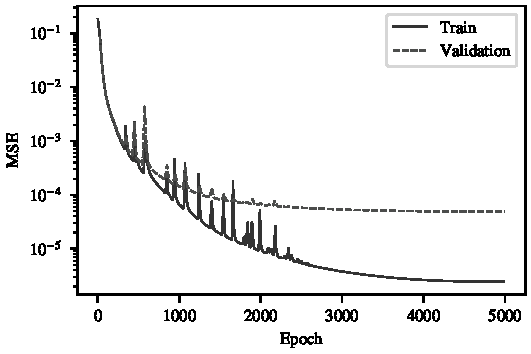
\includegraphics[width=0.5\linewidth]{fig/p3/loss_plot.pdf}
    \caption[Training convergence]{Train and validation loss for the duration of the experiment.}
    \label{fig:convergence}
\end{figure}

\subsection{Derivative calculation}
A naive approach to calculating gradients with the trained INR would be to evaluate the representation \(f(x, y, z)\) at a set of coordinates \({(x, y, z)}_1 \dots {(x,y,z)}_n\), and use numerical differentiation with the output grid to calculate derivatives.
However, using AD with Pytorch, the implicit representation can be differentiated with respect to its coordinate inputs to provide spatial gradients, prior to being queried at the nodes of a quantised grid.
That is, to directly sample \(\nabla{}\phi{}_{(x,y,z)}\) at \({(x, y, z)}_1 \dots {(x,y,z)}_n\).
%TODO we dont show these Higher orders - should we?
Higher order derivatives are calculated using AD in the same manner.

\section{Results}
\subsection{Level grid prediction from INR}
Querying a learnt INR using a regularly spaced \(x,y\) grid at a specific \(z\) height is a novel method for producing level grids from geophysical potential field surveys.
The cell size can be selected using a finer or coarser \(x,y\) spacing, including variable or anisotropic cell sizes.
Contemporary super-resolution research can leverage this continual representation as a framework for high quality arbitrary scale factor high-frequency signal prediction \parencite[e.g][]{chenLearningContinuousImage2021}.
However, the potential field representation task here does not attempt to predict additional high-frequency information and resolution remains determined by the survey sample spacing and neural network capacity.

\Cref{fig:grid} shows the INR queried at \(z=\SI{40}{\meter}\), which is the nominal terrain clearance of the survey.
A good qualitative match is achieved between the GA reference grid and the grid queried from the implicit representation, which successfully reconstructs the linear dune features and circular rim features.
This high performance is quantified by the residuals and peak signal to noise ratio (PSNR) of \SI{40.12}{\dB}.
% Further level grids from other survey extents are included in Appendix A.

\begin{figure}[hbt]
    \centering{}
    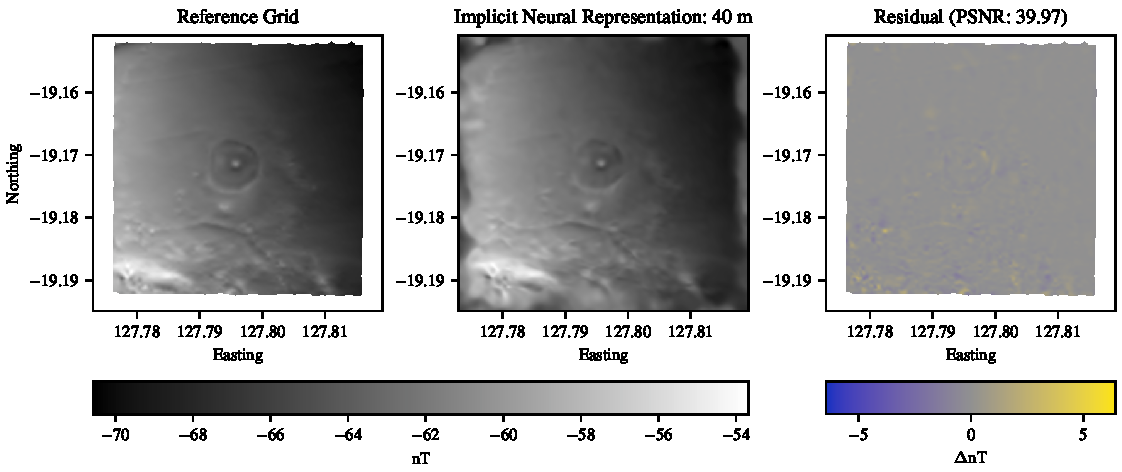
\includegraphics[width=1.0\linewidth]{fig/p3/P864_grid_comparison_40m.pdf}
    \caption[Grid prediction (40 m)]{Comparison between the reference grid processed by Geoscience Australia (left) and the constant level grid queried from the INR at \SI{40}{\m} (middle). The residuals are shown for areas containing reference data (right), with a range of ±2 standard deviations of values in the reference grid.}
    \label{fig:grid}
\end{figure}

The INR can be queried at arbitrary continuous coordinates, including out-of-range values beyond the training domain.
As expected, the predicted field becomes unrealistic when extrapolating beyond this boundary, which can be seen in the periphery of the INR grid in \cref{fig:grid}.
This boundary region (indicated by solid white in the reference grid) is excluded from PSNR calculation.

Constant level grids can be queried from the INR at any height.
\Cref{fig:grid35} shows the case study INR queried at \SI{35}{\m}, which is \SI{5}{\m} lower than the nominal survey altitude.
While the rim feature can still be interpreted within this lower level grid, the INR fails to demonstrate physically realistic continuation of the field.
% It is conjectured that successfully training a PINN criterion such as Laplace’s equation loss (equation 1.3) would improve the accuracy of these upward or downward extracted slices. 

\begin{figure}[hbt]
    \centering{}
    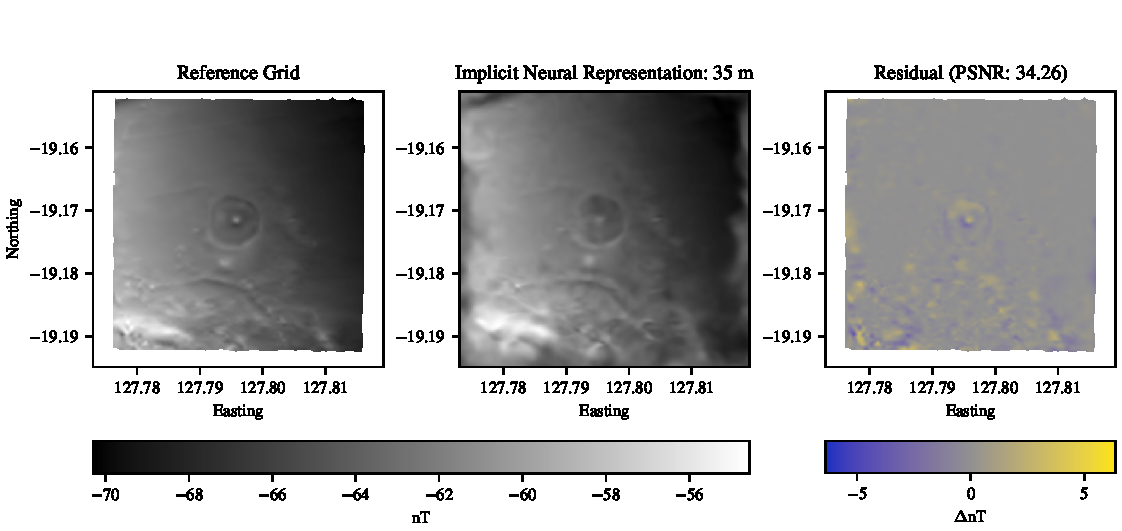
\includegraphics[width=1.0\linewidth]{fig/p3/P864_grid_comparison_35m.pdf}
    \caption[Grid prediction (35 m)]{A constant level grid queried from the INR at the height of \SI{35}{\m} (middle).}
    % AWAGS is 80 m, but we see nothing useful at 80m
    \label{fig:grid35}
\end{figure}

% The strong performance of the model is retained even when using a subsampled training dataset, here shown at \qty{30}{\percent} and \qty{10}{\percent} (\cref{fig:gridpct}) of the total available data.
% % In both cases, the validaiton and test sets remain identical to the initial training split.

% \begin{figure}[hbt]
%     % \includegraphics[]{fig/p3/grid_subpct.pdf}
%     \caption[Grid subsampled]{Performance of level grid prediction shown at \qty{30}{\percent} and \qty{10}{\percent} random sampling of training data.}
%     \label{fig:gridpct}
% \end{figure}


\subsection{Spatial derivatives and filters}
Using AD, derivatives can be calculated between the input spatial coordinates and the output potential field representation.
While horizontal derivatives queried from the INR correspond well to numerical derivatives calculated on the \SI{40}{\m} level grid in \cref{fig:hori_grad}, the vertical derivative suffers poor performance \cref{fig:vert_grad}.
This correlates with the poor continuation performance of model when predicting level grids several meters or more beyond the nominal sample height.
This is interpreted as the presented model having a limited capacity to extrapolate, and learning a poor representation of the vertical component of the potential field, which we further discuss in \cref{sec:discussion}

\begin{figure}[hbt]
    \centering{}
    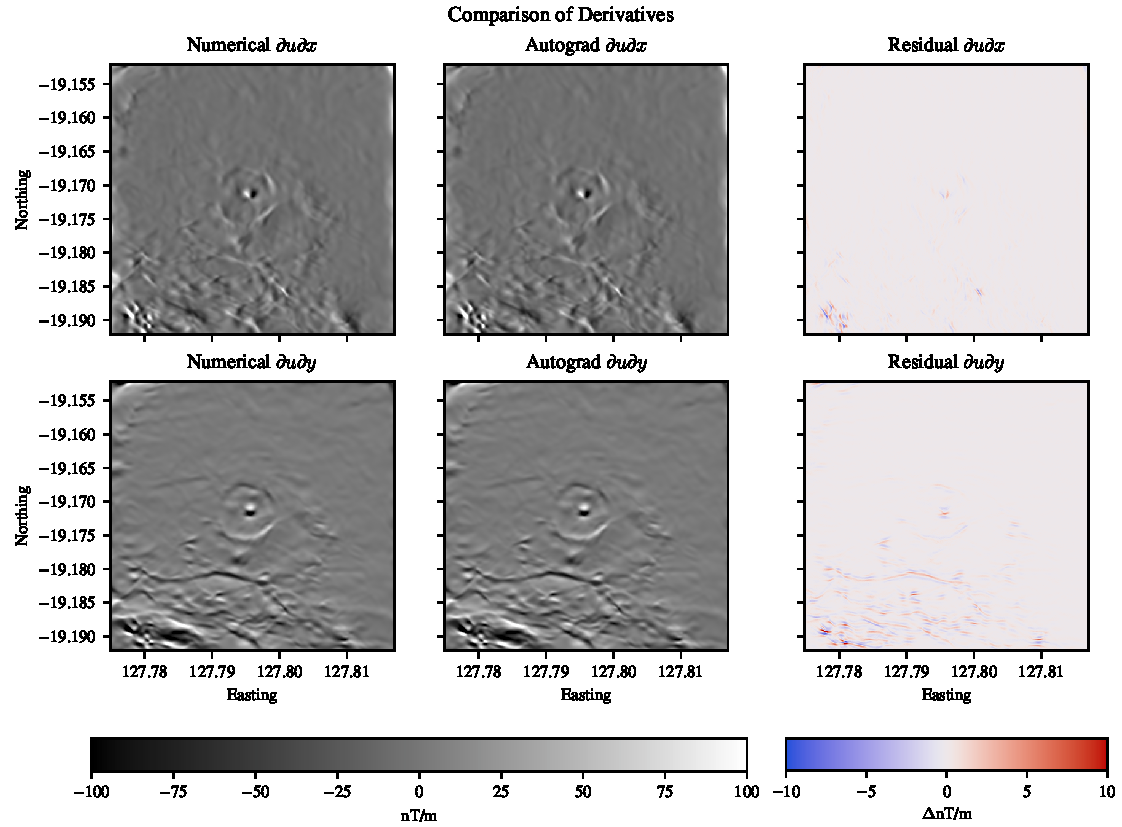
\includegraphics[width=1.0\linewidth]{fig/p3/P864_dh_comparison.pdf}
    \caption[Horizontal derivatives]{Horizontal gradients calculated using the proposed method and the reference numerical method.
        Both numerical differentiaion (left column) and AD INR (middle column) are calculated on the INR level grid or INR respectively.
        Residuals are calculated between the numerical and AD gradient grids (right column).}
    \label{fig:hori_grad}
\end{figure}

\begin{figure}[hbt]
    \centering{}
    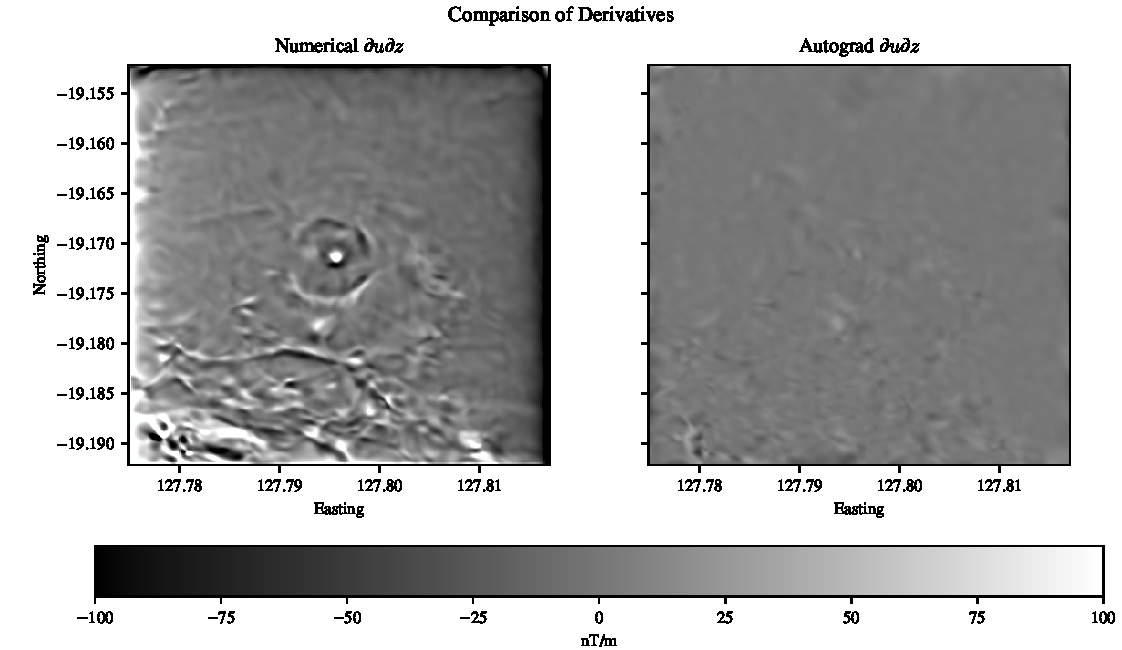
\includegraphics[width=1.0\linewidth]{fig/p3/P864_dv_comparison.pdf}
    \caption[Vertical derivative]{Vertical derivative grids queried from AD differentiated INR (left) and calculated numerically (right) on the \SI{40}{m} level grid queried from the INR\@. The proposed method has poor vertical gradient representation, possibly due to the nature of aeromagnetic survey design.}
    \label{fig:vert_grad}
\end{figure}

\section{Discussion}
\label{sec:discussion}
The proposed method has strong learning capacity for the potential field samples in the horizontal plane near the nominal survey altitude, allowing extraction of level grids which are accurate against the reference grid.
Level grids can be queried at arbitrary heights and cell sizes, with the highest accuracy achieved at the realised nominal survey altitude.
Performance decreases within approximately one standard deviation from that height (\SI{35} to \SI{45}{\m}), with gradual failure of the model outside of that range.
It is interpreted from the poor quality of the vertical gradients and out-of-range level grid predictions that the model is learning a function between horizontally coplanar points, and not an accurate vertical continuation function.
This is conjectured to be caused by aeromagnetic sampling being carried out on a nominally horizontal planar drape surface, without sufficient repeat measurements at other heights to train the network for the vertical field component.

While quantised grids can be queried at any cell size, short wavelength information beyond the Nyquist limit of the survey line sampling is not predicted.
The current method could include additional target dimensions, which would allow representation learning of vector fields \(\mathbb{R}^{3}\) in three dimensions \(\mathbb{R}^{3}\).
This has applications in tensor fields and data integration tasks, and these remain for future work.

INR is a rapidly evolving field of research, and draws on contemporary established deep learning improvements within related fields.
In addition to improving the high-frequency learning capacity with novel activation functions and regularisation methods, fundamental neural network research and hardware development is ongoing.

% Even when using a small subset of the dataset, this performance is retained.

% The case study survey presented is very small compared to typical regional aeromagnetic surveys.
% A demonstration of the method on a large aeromagnetic survey, requiring minibatch training, is included in \cref{app:menzies}.
% Training of this representation follows the parameters outlined in \cref{sec:training}, which were optimised for the Wolfe Creek case study, with the addition of a shuffled minibatch size of \SI{1024000}\@.
% Attempts to train the CMLP with small batch sizes did not converge.%, reflecting the non-convergence result found for training on very large subsampling factors of the line dataset.


\subsection{Future Work}
\label{sec:future}
The outputs of neural networks can be constrained to obey geophysical laws, using physics-informed neural networks (PINNs) \parencite{raissiPhysicsinformedNeuralNetworks2019}.
PINNs recognise that if the inputs to a neural network are samples of a function which follows some physical law, outputs from the model should similarly be constrained by that law.
By regularising the network with an objective function which penalises solutions that don't fit the partial differential equations describing the law, it is possible to vastly reduce the physically valid solution search space \parencite{raissiPhysicsinformedNeuralNetworks2019}.
Because CMLP networks with periodic activations are continuously differentiable, it is possible to enforce this constraint as an element of the overall loss function within the network.
\Textcite{sethiHardEnforcementPhysicsinformed2023} demonstrate that this regularisation does not have to be implemented as a loss function, but instead can be a hard constraint embedded within the network.
Another approach \parencite{liImplicitStochasticGradient2023} replaces the ubiquitous stochastic gradient descent optimiser \emph{Adam} with an implicit stochastic gradient descent (ISGD) method.

Examples of physics-informed constraints include enforcing initial or boundary conditions, or conforming to known properties of the modelled signal.
Potential fields in an airborne sampling context are constrained by a number of physical laws, including \emph{Laplace's equation};
\[
    \nabla^2 \phi = 0,
\]
or denoted in three dimensions,
\begin{equation}
    \label{eqn:Laplace}
    \frac{\partial{}^2\phi}{\partial{}x^2} + \frac{\partial{}^2\phi}{\partial{}y^2} + \frac{\partial{}^2\phi}{\partial{}z^2} = 0.
\end{equation}
Inspired by the approach of \cite{raissiPhysicsinformedNeuralNetworks2019}, a geophysics informed network could include a Laplace criterion,

\begin{equation}
    \label{eqn:cri_laplace}
    \mathcal{L}_{PDE} = \frac{1}{S_i}\sum_{i=1}^{S_i} \left(\frac{\partial{}^2f}{\partial{}x^2} + \frac{\partial{}^2f}{\partial{}y^2} + \frac{\partial{}^2f}{\partial{}z^2}\right)^2,
\end{equation}
where \(S_i\) indicates the \(i^{th}\) sample point of the field survey \(\phi(x, y, z)\).
This criterion penalises outputs where Laplace's equation is not satisfied because the sum of partial second derivatives is not close to zero.

%     \mathcal{L}_{PDE} = \lVert{}\frac{\partial{}^2f}{\partial{}x^2} + \frac{\partial{}^2f}{\partial{}y^2} + \frac{\partial{}^2f}{\partial{}z^2}\rVert{}_{2}
%TODO Confirm logic here: % If Laplace's equation:\( \nabla^2 \phi = 0 \) is satisfied, it is harmonic, and has continuous single valued first derivatives, and has second derivatives.
% This indicates the function lacks curvature. 
% Blakely:
% A force field \(F\) is the gradient (or negative gradient) of the potential energy.
% \( F = \nabla\phi \) for the gravity potential, \(F = - \nabla \phi\) for the Magnetic potential.
% \( \phi(x,y,z) = constant \) is an equipotential surface.
% Numerical methods for potential field continuation are unstable, recognised in the geophysical community by solution divergence and noise in predictions.

Initial attempts using the objective function approach were trialled in this work, but failed to converge and remain for future work.
Other geophysical formulae may present avenues for PINN implementation, such as vertical continuation described in \cite{blakelyPotentialTheoryGravity1996}.

\section{Conclusions}
High-resolution implicit neural representation of potential field geophysics surveys is achieved with the use of coordinate MLP neural networks for INR.
Resolution in the representation is limited by network capacity, rather than initial grid cell size selection during regularisation.
Level grids can be extracted from these representations, emerging as a novel method for regularising scattered geophysical sample data.
Gradients can be calculated using the learnt representation, and gridded \emph{a posteri} of gradient calculation.

\section{Acknowledgements}
This project is funded by a Rio Tinto Iron Ore PhD scholarship.

\printbibliography{}

% \section{Appendix A}
% \label{app:menzies} %TODO format as "Appendix"
% The Menzies North P864 survey contains xxx sample points across yyyy line kilometres, and was flown at a nominal terrain clearance of zz m.
% While a high-quality result is attainable using batch gradient descent on a subset of the survey points, minibatch gradient descent is demonstrated for the CMLP used to learn the full survey INR\@.


% \begin{figure}[hbt]
%     % \includegraphics[width=\textwidth]{fig/p3/menzies.pdf}    
%     \caption[Menzies INR]{Level grid representation using minibatch gradient descent.}
%     \label{fig:vert_grad}
% \end{figure}


\end{document}